\documentclass{beamer}
\setbeamertemplate{caption}[numbered]
\usetheme{CambridgeUS}
 %\usetheme{Berlin}
% \usetheme{Copenhagen}
% \usetheme{AnnArbor}
% \usetheme{Antibes}
% \usetheme{Bergen}
\usepackage{graphicx} % Required for inserting images
\usepackage{tikz}
\usepackage{wrapfig}
\usepackage{tcolorbox}
\usepackage{caption}

\title[E\&M: an Approach using GFD and FEM]{A Comparison between a Novel Algorithm for Finite Differences and the Established Finite Element Method to Simple Electrostatic Potentials}

\author[]{Hayden P. Scholz \inst{1} \and J. Emmanuel Flores \inst{1} \and Cullen M. Sullivan\inst{1}}

\institute[Tufts University]{\inst{1} Tufts University, Medford, MA}

\date{\today}
% logo of my university
\titlegraphic{\includegraphics[width=4cm]{Figures/A&S_Hori_BK+BL.jpg}}

\AtBeginSection[] % Show Outline at the beginning of every new section.
{
    \begin{frame}
        \frametitle{Table of Contents}
        \tableofcontents[currentsection]
    \end{frame}
}

\begin{document}

\maketitle

\begin{frame}
\frametitle{Outline}
  \tableofcontents
\end{frame}
% \begin{frame}{Outline}
%   \tableofcontest
% \end{frame}
\section{Introduction}

\subsection{Physics and PDE}
\begin{frame}{Physics and PDE}
    \begin{columns}
        \begin{column}{0.6\textwidth}
            \begin{itemize}
                \item<1-> Almost all of the physical laws are written in the language of PDEs.
                \item<2-> The huge complexity of these equations make them difficult(or impossible) to solve analytically.
                \item<3-> Numerical Methods:
                    \begin{itemize}
                        \item<4-> Finite Differences
                        \item<5-> Finite Element (Volume) Methods.
                        \item<5-> Spectral Methods (Chebyshev polynomials).
                    \end{itemize}
            \end{itemize}
        \end{column}
        \begin{column}{0.37\textwidth}
            \begin{tcolorbox}[title= Maxwell's Equations]
            \begin{itemize}
                \item $\nabla\cdot \mathbf{E} =\rho / \epsilon_0,$
                \item $\nabla\times \mathbf{E} = 0, $
                \item $\nabla\cdot \mathbf{B} = 0,$
                \item $\nabla\times \mathbf{B} = \mu_0\mathbf{J}.$
            \end{itemize}
            \end{tcolorbox}
        \end{column}
    \end{columns}    
\end{frame}



\section{Problem studied: Coaxial Cable}

\subsection{Statement of the Problem}

\begin{frame}{Statement of the Problem}
\begin{columns}
    \begin{column}{0.6\textwidth}
    \begin{itemize}
        \item Coaxial Cylinders
        \begin{itemize}
            \item Radial symmetry
            \item Analytic solution is nonlinear
        \end{itemize}
    \end{itemize}
    \end{column}
    \begin{column}{0.4\textwidth}  %%<--- here
        \begin{center}
            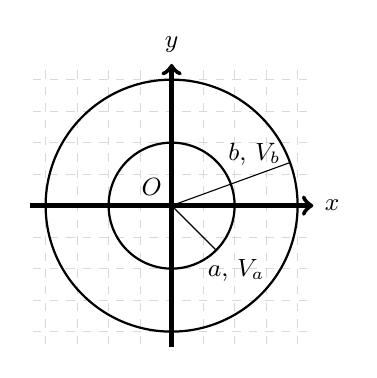
\begin{tikzpicture} [scale=0.40]    
            \draw[help lines, color=gray!30, dashed] (-4.4,-4.4) grid (4.4,4.4);
            \draw[->,ultra thick] (-4.5,0)--(4.5,0) node[right]{\small $x$};
            \draw[->,ultra thick] (0,-4.5)--(0,4.5) node[above]{\small $y$};
            \draw [thick] circle [radius=2.0];
            \draw [thick] (0,0) circle [radius=4];
            \draw[-, rotate around={-45:(0,0)}] (0,0) -- (2,0)  node [pos=1.45] {\small $a$, $V_a$};
            \draw[-, rotate around={20:(0,0)}] (0,0) -- (4.,0) node [pos=0.7, above] {\small $b$, $V_b$};
            \draw[fill=black](0,0) circle (1 pt) node [anchor=south east] {\small $O$};
            \end{tikzpicture}
            \captionof{figure}{Two dimensional schematic projection of the coaxial problem.}
         \end{center}
    \end{column}
\end{columns}
\end{frame}

\subsection{Analytical Solution}

\begin{frame}{Analytical Solution}
\begin{columns}
\begin{column}{0.6\textwidth}
\begin{itemize}
    \item<1-> Laplacian in Cylindrical Coordinates
    \begin{equation}
    \frac{1}{r}\frac{\partial}{\partial r}\left(r\frac{\partial V}{\partial r}\right) + \frac{1}{r^2}\frac{\partial^2 V}{\partial \theta^2} + \frac{\partial^2 V}{\partial z^2} = 0,
    \end{equation}
    \item<2-> Simplification by symmetry
    \begin{equation}
    \frac{1}{r}\frac{\partial}{\partial r}\left(r\frac{\partial V}{\partial r}\right)=0,
    \end{equation}
    \item<3-> Analytical Solution
    \begin{equation}
    V(r) = \frac{V_b - V_a}{\ln(b/a)}\ln\left(\frac{r}{a}\right) + V_a.
    \label{eq:coax_pot}
    \end{equation}
\end{itemize}
\end{column}
    \begin{column}{0.4\textwidth}  %%<--- here
        \begin{center}
            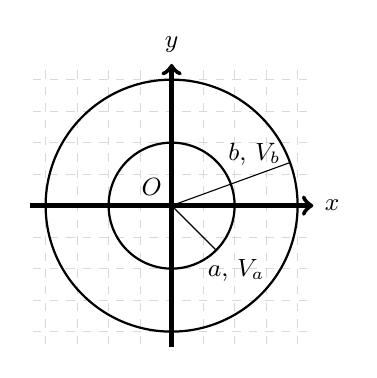
\begin{tikzpicture} [scale=0.40]    
            \draw[help lines, color=gray!30, dashed] (-4.4,-4.4) grid (4.4,4.4);
            \draw[->,ultra thick] (-4.5,0)--(4.5,0) node[right]{\small $x$};
            \draw[->,ultra thick] (0,-4.5)--(0,4.5) node[above]{\small $y$};
            \draw [thick] circle [radius=2.0];
            \draw [thick] (0,0) circle [radius=4];
            \draw[-, rotate around={-45:(0,0)}] (0,0) -- (2,0)  node [pos=1.45] {\small $a$, $V_a$};
            \draw[-, rotate around={20:(0,0)}] (0,0) -- (4.,0) node [pos=0.7, above] {\small $b$, $V_b$};
            \draw[fill=black](0,0) circle (1 pt) node [anchor=south east] {\small $O$};
            \end{tikzpicture}
            \captionof{figure}{Two dimensional schematic projection of the coaxial problem.}
         \end{center}
    \end{column}
    \end{columns}
\end{frame}

\section{Computational Setup}
\subsection{General Finite Differences Method}
\begin{frame}{Finite Differences Methods}
\begin{columns}
    \begin{column}{0.6\textwidth}
        \begin{itemize}
            \item <1-> How can we approximate the Laplacian operator?
            \begin{equation*}
                \nabla^2 \xrightarrow{Discretize} \;\;\; ???
            \end{equation*}
            \item <2-> Use a quotient to approximate partial derivatives
            \begin{equation}
                \frac{\partial^2 V}{\partial x^2} \approx \frac{1}{2} \frac{\Delta V}{(\Delta x)^2}
            \end{equation}
            \item<2-> We can model a system with a series of these \textbf{finite differences} to approximate a partial differential operator
        \end{itemize}
    \end{column}
    \begin{column}{0.4\textwidth}
        % \begin{figure}[h]
        %     \centering
        %     \includegraphics[width=0.95\textwidth]{Figures/Landau_FDM.png}
        %     \caption{   (TODO: Cite me.)}
        %     \label{fig:landau_fdm}
        % \end{figure}
%         \begin{tikzpicture}
% [
%   xscale=0.8,
%   yscale=0.8,
%   grid/.style={draw,thin,gray!50},
%   node/.style={draw,circle,fill=black,inner sep=1pt}
% ]

% % Grid lines
% \draw[grid] (0,0) grid (4.5,4.4);
% \draw[help lines, color=gray!30, dashed] (-0.5,-0.5) grid (4.4,4.4);
% \draw[->,ultra thick] (-0.25,-0.25)--(4.5,-0.25) node[right]{$x$};
% \draw[->,ultra thick] (-0.25,-0.26)--(-0.25,4.5) node[above]{$y$};

% % Grid points
% \foreach \x in {0,1,2,3,4} {
%   \foreach \y in {0,1,2,3,4} {
%     \node [node] at (\x,\y) {};
%   }
% }

% \end{tikzpicture}

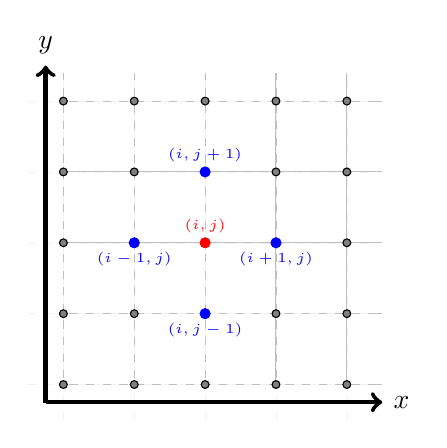
\begin{tikzpicture}
[
  xscale=0.9,
  yscale=0.9,
  grid/.style={draw,thin,gray!50},
  node/.style={draw,circle,fill=gray,inner sep=1pt}
]

% Grid lines
\draw[grid] (0,0) grid (4.5,4.4);
\draw[help lines, color=gray!10, dashed] (-0.5,-0.5) grid (4.4,4.4);
\draw[->,ultra thick] (-0.25,-0.25)--(4.5,-0.25) node[right]{$x$};
\draw[->,ultra thick] (-0.25,-0.26)--(-0.25,4.5) node[above]{$y$};

% Grid points
\foreach \x in {0,1,2,3,4} {
  \foreach \y in {0,1,2,3,4} {
    \node [node] at (\x,\y) {};
  }
}
\filldraw[red] (2,2) circle (2pt) node[anchor=south]{\tiny $(i,j)$};
\filldraw[blue] (3,2) circle (2pt) node[anchor=north]{\tiny $(i+1,j)$};
\filldraw[blue] (1,2) circle (2pt) node[anchor=north]{\tiny $(i-1,j)$};
\filldraw[blue] (2,3) circle (2pt) node[anchor=south]{\tiny $(i,j+1)$};
\filldraw[blue] (2,1) circle (2pt) node[anchor=north]{\tiny $(i,j-1)$};

\end{tikzpicture}
    \end{column}
\end{columns}
\end{frame}

\begin{frame}{Generalizing Finite Differences}
\begin{columns}
    \begin{column}{0.6\textwidth}
        \begin{itemize}
            \item <1-> Express FDM on an arbitrary graph (mesh)
            \item <1-> Every node wants to satisfy Laplace's equation,
            \begin{equation}
                \nabla^2 V_i = 0
            \end{equation}
            \item <2-> Using a finite differences approximation, every node is informed by its neighbors
            \item <2-> Fix potential of some nodes (boundary conditions), then generate a linear system of equations that can be solved
        \end{itemize}
    \end{column}
    \begin{column}{0.4\textwidth}
        \begin{figure}[h]
            \centering
            \includegraphics[width=0.95\textwidth]{Figures/Coax_GFDM_Connectivity.png}
            \label{fig:coax_gfdm_connectivity}
            \caption{Schematic of the GFDM approach to the COAX problem. Black nodes are boundaries, lines show connections generated by the GFDM algorithm.}
        \end{figure}
    \end{column}
\end{columns}
\end{frame}

\section{Finite Element Method}
\begin{frame}{FEM Approach}
    \begin{columns}
        \begin{column}{0.5\textwidth}
            \begin{itemize}
            \item<1-> Strong Form: function and its derivatives for a well posed problem.
            \item<2-> What if we expand/relax the conditions?
            \item<3-> Express the problem in a variational way
            \item<4-> Approximate the solution in each element and interpolate solutions.
            \end{itemize}
        \end{column}

        \begin{column}{0.4\textwidth}
            \begin{itemize}
                \item<5-> Weak Form:
                    \begin{equation*}
                        \int_{\Omega}d\Omega( \nabla V\cdot\nabla \eta )= 0
                    \end{equation*}
                \begin{figure}
                    \centering
                    \includegraphics[width=0.75  \textwidth]{Figures/Coaxial_Mesh-removebg-preview.png}
                    \caption{Mesh for the coaxial cable problem.}
                    \label{fig:Coax_Mesh}
                \end{figure}
            \end{itemize}
        \end{column}
    \end{columns}
\end{frame}

\section{Results}

\subsection{GFD and FEM}

\begin{frame}{Coaxial Cable}
\begin{figure}[h]
\begin{columns}
    \begin{column}{0.5\linewidth}
        \centering\includegraphics[width=0.85\textwidth]{Figures/Coax_GFDM.png}
    \end{column}
    \begin{column}{0.5\linewidth}
        \centering\includegraphics[width=1.0\textwidth]{Figures/PotentialFieldFEMCoaxial.png}
    \end{column}
\end{columns}
\caption{
Potential obtained for the coaxial cable. \textbf{Left}: GFD approach. \textbf{Right}: FEM approach. As we can see, we have a qualitatively good agreement between both approaches.}
\label{fig:tCoaxial_Cable_VField}
\end{figure}
\end{frame}

\begin{frame}{Comparison Between Both Approaches}
\begin{figure}[h]
\begin{columns}
    \begin{column}{0.5\linewidth}
        \includegraphics[width=0.95\textwidth]{Figures/ComparissonPotentialFEMGFD.png}
    \end{column}
    \begin{column}{0.5\linewidth}
        \includegraphics[width=0.95\textwidth]{Figures/ComparissonPotentialFEMGFD_Zoom.png}
    \end{column}
\end{columns}
\caption{Comparison between both approaches for the coaxial cable, for GFD we have an RMS = 0.084, whereas for FEM RMS = 0.008. \textbf{Left}: Plot for the whole domain of the radius. \textbf{Right}: Zoom on the zone where the solutions are most different between each other.}
\label{fig:Comparison_GFD_FEM}
\end{figure}
\end{frame}

\begin{frame}
\begin{columns}
    \begin{column}{0.5\linewidth}
    \begin{itemize}
        \item We tried running GFDM on the coaxial problem many times to see if error decreases with higher resolution
        \item Low node count causes noise in the solution
        \item High node count shows a more stable and lower error solution
    \end{itemize}
    \end{column}
    \begin{column}{0.5\linewidth}
    \begin{figure}[h]
        \centering
        \includegraphics[width=0.95\textwidth]{Figures/Coax_GFDM_Nodes_Neighbors_RMS.png}
        \caption{RMS error of many independent GFDM solutions for the coaxial problem.}
        \label{fig:coax_gfdm_nodes_neighbors}
    \end{figure}
    \end{column}
\end{columns}
\end{frame}

% \begin{frame}{FEM: Comparison with the potential field}
%     \begin{figure}
%         \centering
%         \includegraphics[scale=0.4]{Figures/ComparissonPotentialFEMCoaxial.png}
%         \caption{Potential field as function of the radial distance: Comparison between the analytical solution and the approximate solution using FEM.}
%         \label{fig:FEM_V_Sol}
%     \end{figure}
% \end{frame}

% \begin{frame}{GFD vs FEM}
%     \begin{figure}
%         \centering
%         \includegraphics[scale = 0.5]{Figures/ComparissonPotentialFEMGFD.png}
%         \caption{Caption}
%         \label{fig:enter-label}
%     \end{figure}
% \end{frame}

\subsection{Complex Geometries}
% \begin{frame}{Two rectangle bars}
%     \begin{figure}
%         \centering
%         \includegraphics[scale = 0.4]{Figures/TwoBars.png}
%         \caption{Two Bars}
%         \label{fig:enter-label}
%     \end{figure}
% \end{frame}


\begin{frame}{Two conducting bars}
\begin{figure}[h]
\begin{columns}
    \begin{column}{0.5\linewidth}
        \includegraphics[width=0.95\textwidth]{Figures/Bars_GFDM.png}
    \end{column}
    \begin{column}{0.5\linewidth}
        \includegraphics[width=0.95\textwidth]{Figures/Bars_FEM.png}
    \end{column}
\end{columns}
\caption{Two conducting bars each held at 10.0 V with the bounding box grounded. \textbf{Left}: GFDM solution (5822 nodes). \textbf{Right}: FEM solution.}
\label{fig:two_bars}
\end{figure}
\end{frame}

\begin{frame}{Error for two conducting bars}
\begin{columns}
    \begin{column}{0.5\linewidth}
    \begin{itemize}
        \item GFDM solution does well between the conductors
        \item Outside the conductors, the solution is not as good
        \item Solution is sensitive to irregularities in the mesh
    \end{itemize}
    \end{column}
    \begin{column}{0.5\linewidth}
        \begin{figure}[h]
        \includegraphics[width=0.95\textwidth]{Figures/Bars_Error.png}
        \caption{Error (GFDM - FEM) for the two conducting bars problem. RMS = 0.577}
        \label{fig:two_bars_error}
        \end{figure}
    \end{column}
\end{columns}
\end{frame}

\begin{frame}{Conducting dolphin}
\begin{figure}[h]
\begin{columns}
    \begin{column}{0.5\linewidth}
        \includegraphics[width=0.95\textwidth]{Figures/Dolfin_GFDM.png}
    \end{column}
    \begin{column}{0.5\linewidth}
        \includegraphics[width=0.95\textwidth]{Figures/Dolfin_FEM.png}
    \end{column}
\end{columns}
\caption{Ideally conducting dolphin held at 10.0 V with the bottom boundary held at 5.0 V and other boundaries grounded. \textbf{Left}: GFDM solution (2868 nodes). \textbf{Right}: FEM solution.}
\label{fig:dolfin}
\end{figure}
\end{frame}

\begin{frame}{Conducting dolphin error}
\begin{columns}
    \begin{column}{0.5\linewidth}
    \begin{itemize}
        \item Dolphin solution is not very good for GFDM compared to FEM
        \item Reason is unknown, sparseness of points far from the dolphin may be causing a problem
        \item Laplacian approximation failing may be the reason for poor solution throughout
    \end{itemize}
    \end{column}
    \begin{column}{0.5\linewidth}
        \begin{figure}[h]
        \includegraphics[width=0.95\textwidth]{Figures/Dolfin_Error.png}
        \caption{Error (GFDM - FEM) for the two conducting bars problem. RMS = 1.870}
        \label{fig:dolfin_error}
        \end{figure}
    \end{column}
\end{columns}
\end{frame}

\begin{frame}{Conducting python}
\begin{figure}[h]
\begin{columns}
    \begin{column}{0.5\linewidth}
        \centering
        \includegraphics[width=0.80\textwidth]{Figures/Python_GFDM.png}
    \end{column}
    \begin{column}{0.5\linewidth}
        \centering
        \includegraphics[width=0.80\textwidth]{Figures/Python_FEM.png}
    \end{column}
\end{columns}
\caption{Ideally conducting python held at 10.0 V with the bounding box grounded. \textbf{Left:} GFDM solution (2201 nodes). \textbf{Right:} FEM solution.}
\label{fig:python}
\end{figure}
\end{frame}

\begin{frame}{Conducting python error}
\begin{columns}
    \begin{column}{0.5\linewidth}
    \begin{itemize}
        \item Python solution performs well near the snake
        \item Some "hotspots" of error where the solver did not perform well
        \item Points of high error have boundaries that are near each other
        \item Perhaps the solver does not do well for quickly changing potentials
    \end{itemize}
    \end{column}
    \begin{column}{0.5\linewidth}
        \begin{figure}[h]
        \includegraphics[width=0.80\textwidth]{Figures/Python_Error.png}
        \caption{Error (GFDM - FEM) for the two conducting bars problem. RMS = 1.013}        \label{fig:python_error}
        \end{figure}
    \end{column}
\end{columns}
\end{frame}

\section*{Bibliography}
\begin{frame}[allowframebreaks]{Bibliography}

\beamertemplatebookbibitems
\begin{thebibliography}{}
\bibitem{NetworkX}HAGBERC, ARIC, SCHULT, DAN, S. \newblock \textquotedbl NetworkX.\textquotedbl{} \newblock Software Package.

\bibitem{-}Harris, Charles R., et al. \newblock \textquotedbl Array programming with NumPy.\textquotedbl{} \newblock Nature 585.7825 (2020): 357-362.

\bibitem{--}Landau, Rubin H., Manuel J. Páez, and Cristian C. Bordeianu. \newblock \textquotedbl Computational physics: Problem solving with Python\textquotedbl{} \newblock John Wiley & Sons, 2015.

\bibitem{---}LSchlömer, N. \newblock \textquotedbl "pygalmesh: Python interface for CGAL’s meshing tools.\textquotedbl{} \newblock DOI: https://doi. org/10.5281/zenodo 5564818 (2021).

\end{thebibliography}
\end{frame}
\end{document}
